\chapter{Järjestäminen}

\index{jxrjestxminen@järjestäminen}

\key{Järjestäminen}
on keskeinen algoritmiikan ongelma.
Moni tehokas algoritmi
perustuu järjestämiseen,
koska järjestetyn tiedon
käsittely on helpompaa
kuin sekalaisessa järjestyksessä olevan.

Esimerkiksi kysymys ''onko taulukossa kahta samaa
alkiota?'' ratkeaa tehokkaasti järjestämisen avulla.
Jos taulukossa on kaksi samaa alkiota,
ne ovat järjestämisen jälkeen peräkkäin,
jolloin niiden löytäminen on helppoa.
Samaan tapaan ratkeaa myös kysymys
''mikä on yleisin alkio taulukossa?''.

Järjestämiseen on kehitetty monia
algoritmeja, jotka tarjoavat hyviä
esimerkkejä algoritmien suunnittelun tekniikoista.
Tehokkaat yleiset järjestämis\-algoritmit
toimivat ajassa $O(n \log n)$, ja tämä aikavaativuus
on myös monella järjestämistä käyttävällä algoritmilla.

\section{Järjestämisen teoriaa}

Järjestämisen perusongelma on seuraava:
\begin{framed}
\noindent
Annettuna on taulukko, jossa on $n$ alkiota.
Tehtäväsi on järjestää alkiot pienimmästä
suurimpaan.
\end{framed}
\noindent
Esimerkiksi taulukko
\begin{center}
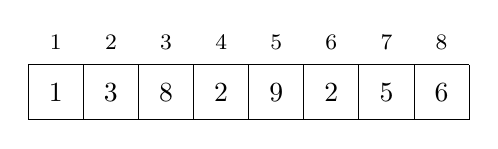
\begin{tikzpicture}[scale=0.7]
\draw (0,0) grid (8,1);
\node at (0.5,0.5) {$1$};
\node at (1.5,0.5) {$3$};
\node at (2.5,0.5) {$8$};
\node at (3.5,0.5) {$2$};
\node at (4.5,0.5) {$9$};
\node at (5.5,0.5) {$2$};
\node at (6.5,0.5) {$5$};
\node at (7.5,0.5) {$6$};

\footnotesize
\node at (0.5,1.4) {$1$};
\node at (1.5,1.4) {$2$};
\node at (2.5,1.4) {$3$};
\node at (3.5,1.4) {$4$};
\node at (4.5,1.4) {$5$};
\node at (5.5,1.4) {$6$};
\node at (6.5,1.4) {$7$};
\node at (7.5,1.4) {$8$};
\end{tikzpicture}
\end{center}
on järjestettynä seuraava:
\begin{center}
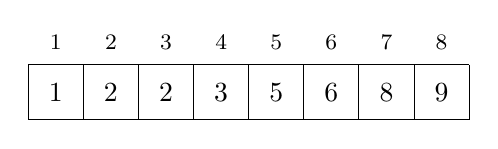
\begin{tikzpicture}[scale=0.7]
\draw (0,0) grid (8,1);
\node at (0.5,0.5) {$1$};
\node at (1.5,0.5) {$2$};
\node at (2.5,0.5) {$2$};
\node at (3.5,0.5) {$3$};
\node at (4.5,0.5) {$5$};
\node at (5.5,0.5) {$6$};
\node at (6.5,0.5) {$8$};
\node at (7.5,0.5) {$9$};

\footnotesize
\node at (0.5,1.4) {$1$};
\node at (1.5,1.4) {$2$};
\node at (2.5,1.4) {$3$};
\node at (3.5,1.4) {$4$};
\node at (4.5,1.4) {$5$};
\node at (5.5,1.4) {$6$};
\node at (6.5,1.4) {$7$};
\node at (7.5,1.4) {$8$};
\end{tikzpicture}
\end{center}

\subsubsection{$O(n^2)$-algoritmit}

\index{kuplajxrjestxminen@kuplajärjestäminen}

Yksinkertaiset algoritmit taulukon
järjestämiseen vievät aikaa $O(n^2)$.
Tällaiset algoritmit ovat lyhyitä ja
muodostuvat tyypillisesti
kahdesta sisäkkäisestä silmukasta.
Tunnettu $O(n^2)$-aikainen algoritmi on
\key{kuplajärjestäminen},
jossa alkiot ''kuplivat'' eteenpäin taulukossa
niiden suuruuden perusteella.

Kuplajärjestäminen muodostuu $n-1$ kierroksesta,
joista jokainen käy taulukon läpi vasemmalta oikealle.
Aina kun taulukosta löytyy kaksi vierekkäistä
alkiota, joiden järjestys on väärä, algoritmi
korjaa niiden järjestyksen.
Algoritmin voi toteuttaa seuraavasti
taulukolle
$\texttt{t}[1],\texttt{t}[2],\ldots,\texttt{t}[n]$:
\begin{lstlisting}
for (int i = 1; i <= n-1; i++) {
    for (int j = 1; j <= n-i; j++) {
        if (t[j] > t[j+1]) swap(t[j],t[j+1]);
    }
}
\end{lstlisting}

Algoritmin ensimmäisen kierroksen jälkeen suurin
alkio on paikallaan, toisen kierroksen jälkeen
kaksi suurinta alkiota on paikallaan, jne.
Niinpä $n-1$ kierroksen jälkeen koko taulukko
on järjestyksessä.

Esimerkiksi taulukossa

\begin{center}
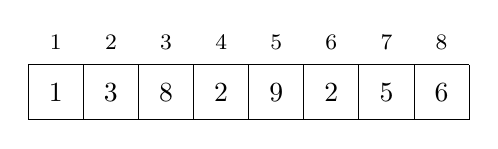
\begin{tikzpicture}[scale=0.7]
\draw (0,0) grid (8,1);

\node at (0.5,0.5) {$1$};
\node at (1.5,0.5) {$3$};
\node at (2.5,0.5) {$8$};
\node at (3.5,0.5) {$2$};
\node at (4.5,0.5) {$9$};
\node at (5.5,0.5) {$2$};
\node at (6.5,0.5) {$5$};
\node at (7.5,0.5) {$6$};

\footnotesize
\node at (0.5,1.4) {$1$};
\node at (1.5,1.4) {$2$};
\node at (2.5,1.4) {$3$};
\node at (3.5,1.4) {$4$};
\node at (4.5,1.4) {$5$};
\node at (5.5,1.4) {$6$};
\node at (6.5,1.4) {$7$};
\node at (7.5,1.4) {$8$};
\end{tikzpicture}
\end{center}

\noindent
kuplajärjestämisen ensimmäinen
läpikäynti tekee seuraavat vaihdot:

\begin{center}
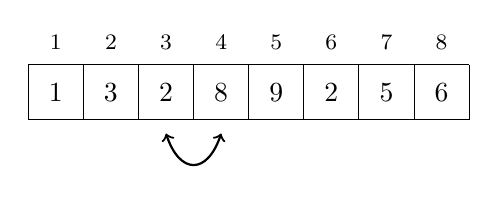
\begin{tikzpicture}[scale=0.7]
\draw (0,0) grid (8,1);
\node at (0.5,0.5) {$1$};
\node at (1.5,0.5) {$3$};
\node at (2.5,0.5) {$2$};
\node at (3.5,0.5) {$8$};
\node at (4.5,0.5) {$9$};
\node at (5.5,0.5) {$2$};
\node at (6.5,0.5) {$5$};
\node at (7.5,0.5) {$6$};

\draw[thick,<->] (3.5,-0.25) .. controls (3.25,-1.00) and (2.75,-1.00) .. (2.5,-0.25);

\footnotesize
\node at (0.5,1.4) {$1$};
\node at (1.5,1.4) {$2$};
\node at (2.5,1.4) {$3$};
\node at (3.5,1.4) {$4$};
\node at (4.5,1.4) {$5$};
\node at (5.5,1.4) {$6$};
\node at (6.5,1.4) {$7$};
\node at (7.5,1.4) {$8$};
\end{tikzpicture}
\end{center}

\begin{center}
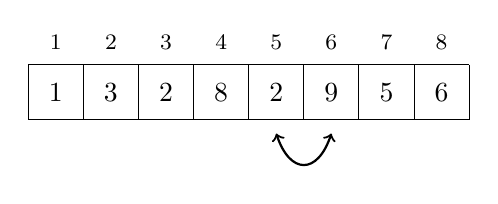
\begin{tikzpicture}[scale=0.7]
\draw (0,0) grid (8,1);
\node at (0.5,0.5) {$1$};
\node at (1.5,0.5) {$3$};
\node at (2.5,0.5) {$2$};
\node at (3.5,0.5) {$8$};
\node at (4.5,0.5) {$2$};
\node at (5.5,0.5) {$9$};
\node at (6.5,0.5) {$5$};
\node at (7.5,0.5) {$6$};

\draw[thick,<->] (5.5,-0.25) .. controls (5.25,-1.00) and (4.75,-1.00) .. (4.5,-0.25);


\footnotesize
\node at (0.5,1.4) {$1$};
\node at (1.5,1.4) {$2$};
\node at (2.5,1.4) {$3$};
\node at (3.5,1.4) {$4$};
\node at (4.5,1.4) {$5$};
\node at (5.5,1.4) {$6$};
\node at (6.5,1.4) {$7$};
\node at (7.5,1.4) {$8$};
\end{tikzpicture}
\end{center}

\begin{center}
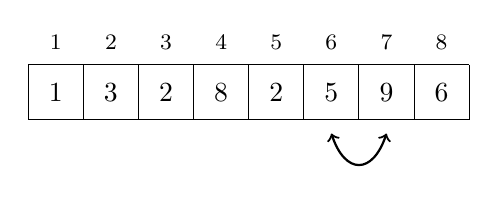
\begin{tikzpicture}[scale=0.7]
\draw (0,0) grid (8,1);
\node at (0.5,0.5) {$1$};
\node at (1.5,0.5) {$3$};
\node at (2.5,0.5) {$2$};
\node at (3.5,0.5) {$8$};
\node at (4.5,0.5) {$2$};
\node at (5.5,0.5) {$5$};
\node at (6.5,0.5) {$9$};
\node at (7.5,0.5) {$6$};

\draw[thick,<->] (6.5,-0.25) .. controls (6.25,-1.00) and (5.75,-1.00) .. (5.5,-0.25);


\footnotesize
\node at (0.5,1.4) {$1$};
\node at (1.5,1.4) {$2$};
\node at (2.5,1.4) {$3$};
\node at (3.5,1.4) {$4$};
\node at (4.5,1.4) {$5$};
\node at (5.5,1.4) {$6$};
\node at (6.5,1.4) {$7$};
\node at (7.5,1.4) {$8$};
\end{tikzpicture}
\end{center}

\begin{center}
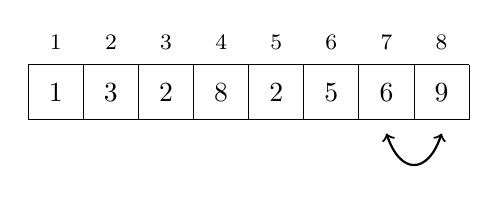
\begin{tikzpicture}[scale=0.7]
\draw (0,0) grid (8,1);
\node at (0.5,0.5) {$1$};
\node at (1.5,0.5) {$3$};
\node at (2.5,0.5) {$2$};
\node at (3.5,0.5) {$8$};
\node at (4.5,0.5) {$2$};
\node at (5.5,0.5) {$5$};
\node at (6.5,0.5) {$6$};
\node at (7.5,0.5) {$9$};

\draw[thick,<->] (7.5,-0.25) .. controls (7.25,-1.00) and (6.75,-1.00) .. (6.5,-0.25);

\footnotesize
\node at (0.5,1.4) {$1$};
\node at (1.5,1.4) {$2$};
\node at (2.5,1.4) {$3$};
\node at (3.5,1.4) {$4$};
\node at (4.5,1.4) {$5$};
\node at (5.5,1.4) {$6$};
\node at (6.5,1.4) {$7$};
\node at (7.5,1.4) {$8$};
\end{tikzpicture}
\end{center}

\subsubsection{Inversiot}

\index{inversio@inversio}

Kuplajärjestäminen on esimerkki algoritmista,
joka perustuu taulukon vierekkäisten alkioiden
vaihtamiseen keskenään.
Osoittautuu, että tällaisen algoritmin
aikavaativuus on \emph{aina} vähintään $O(n^2)$,
koska pahimmassa tapauksessa taulukon
järjestäminen vaatii $O(n^2)$ alkioparin vaihtamista.

Hyödyllinen käsite järjestämisalgoritmien
analyysissa on \key{inversio}.
Se on taulukossa oleva alkiopari
$(\texttt{t}[a],\texttt{t}[b])$,
missä $a<b$ ja $\texttt{t}[a]>\texttt{t}[b]$
eli alkiot ovat väärässä järjestyksessä taulukossa.
Esimerkiksi taulukon
\begin{center}
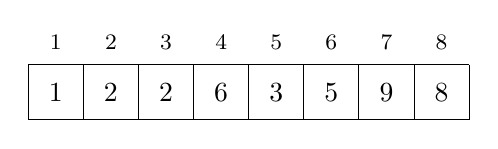
\begin{tikzpicture}[scale=0.7]
\draw (0,0) grid (8,1);
\node at (0.5,0.5) {$1$};
\node at (1.5,0.5) {$2$};
\node at (2.5,0.5) {$2$};
\node at (3.5,0.5) {$6$};
\node at (4.5,0.5) {$3$};
\node at (5.5,0.5) {$5$};
\node at (6.5,0.5) {$9$};
\node at (7.5,0.5) {$8$};

\footnotesize
\node at (0.5,1.4) {$1$};
\node at (1.5,1.4) {$2$};
\node at (2.5,1.4) {$3$};
\node at (3.5,1.4) {$4$};
\node at (4.5,1.4) {$5$};
\node at (5.5,1.4) {$6$};
\node at (6.5,1.4) {$7$};
\node at (7.5,1.4) {$8$};
\end{tikzpicture}
\end{center}
inversiot ovat $(6,3)$, $(6,5)$ ja $(9,8)$.
Inversioiden määrä kuvaa, miten lähellä
järjestystä taulukko on.
Taulukko on järjestyksessä tarkalleen
silloin, kun siinä ei ole yhtään inversiota.
Inversioiden määrä on puolestaan suurin,
kun taulukon järjestys on käänteinen,
jolloin inversioita on
\[1+2+\cdots+(n-1)=\frac{n(n-1)}{2} = O(n^2).\]

Jos vierekkäiset taulukon alkiot
ovat väärässä järjestyksessä,
niiden järjestyksen korjaaminen
poistaa taulukosta tarkalleen yhden inversion.
Niinpä jos järjestämisalgoritmi pystyy
vaihtamaan keskenään vain
taulukon vierekkäisiä alkioita,
jokainen vaihto voi poistaa enintään yhden inversion
ja algoritmin aikavaativuus on varmasti ainakin $O(n^2)$.

\subsubsection{$O(n \log n)$-algoritmit}

\index{lomitusjxrjestxminen@lomitusjärjestäminen}

Taulukon järjestäminen on mahdollista
tehokkaasti ajassa $O(n \log n)$
algoritmilla, joka ei rajoitu vierekkäisten
alkoiden vaihtamiseen.
Yksi tällainen algoritmi on
\key{lomitusjärjestäminen},
joka järjestää taulukon
rekursiivisesti jakamalla sen
pienemmiksi osataulukoiksi.

Lomitusjärjestäminen järjestää taulukon välin
$[a,b]$ seuraavasti:

\begin{enumerate}
\item Jos $a=b$, älä tee mitään, koska väli on valmiiksi järjestyksessä.
\item Valitse välin jakokohdaksi $k=\lfloor (a+b)/2 \rfloor$.
\item Järjestä rekursiivisesti välin $[a,k]$ alkiot.
\item Järjestä rekursiivisesti välin $[k+1,b]$ alkiot.
\item \emph{Lomita} järjestetyt välit $[a,k]$ ja $[k+1,b]$
järjestetyksi väliksi $[a,b]$.
\end{enumerate}

Lomitusjärjestämisen tehokkuus perustuu siihen,
että se puolittaa joka askeleella välin kahteen osaan.
Rekursiosta muodostuu yhteensä $O(\log n)$ tasoa
ja jokaisen tason käsittely vie aikaa $O(n)$.
Kohdan 5 lomittaminen on mahdollista ajassa $O(n)$,
koska välit $[a,k]$ ja $[k+1,b]$ on jo järjestetty.

Tarkastellaan esimerkkinä seuraavan taulukon
järjestämistä:
\begin{center}
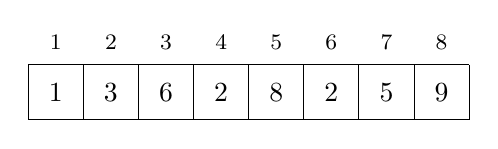
\begin{tikzpicture}[scale=0.7]
\draw (0,0) grid (8,1);
\node at (0.5,0.5) {$1$};
\node at (1.5,0.5) {$3$};
\node at (2.5,0.5) {$6$};
\node at (3.5,0.5) {$2$};
\node at (4.5,0.5) {$8$};
\node at (5.5,0.5) {$2$};
\node at (6.5,0.5) {$5$};
\node at (7.5,0.5) {$9$};

\footnotesize
\node at (0.5,1.4) {$1$};
\node at (1.5,1.4) {$2$};
\node at (2.5,1.4) {$3$};
\node at (3.5,1.4) {$4$};
\node at (4.5,1.4) {$5$};
\node at (5.5,1.4) {$6$};
\node at (6.5,1.4) {$7$};
\node at (7.5,1.4) {$8$};
\end{tikzpicture}
\end{center}

Taulukko jakautuu ensin kahdeksi
osataulukoksi seuraavasti:
\begin{center}
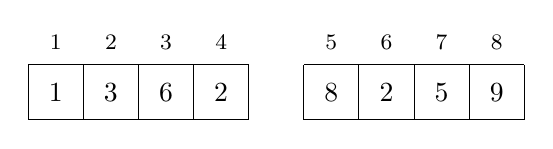
\begin{tikzpicture}[scale=0.7]
\draw (0,0) grid (4,1);
\draw (5,0) grid (9,1);

\node at (0.5,0.5) {$1$};
\node at (1.5,0.5) {$3$};
\node at (2.5,0.5) {$6$};
\node at (3.5,0.5) {$2$};

\node at (5.5,0.5) {$8$};
\node at (6.5,0.5) {$2$};
\node at (7.5,0.5) {$5$};
\node at (8.5,0.5) {$9$};

\footnotesize
\node at (0.5,1.4) {$1$};
\node at (1.5,1.4) {$2$};
\node at (2.5,1.4) {$3$};
\node at (3.5,1.4) {$4$};
\node at (5.5,1.4) {$5$};
\node at (6.5,1.4) {$6$};
\node at (7.5,1.4) {$7$};
\node at (8.5,1.4) {$8$};

\end{tikzpicture}
\end{center}

Algoritmi järjestää osataulukot rekursiivisesti,
jolloin tuloksena on:
\begin{center}
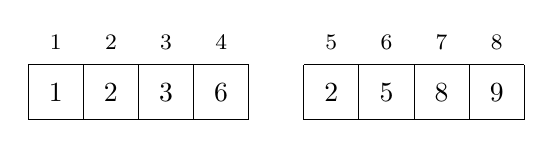
\begin{tikzpicture}[scale=0.7]
\draw (0,0) grid (4,1);
\draw (5,0) grid (9,1);

\node at (0.5,0.5) {$1$};
\node at (1.5,0.5) {$2$};
\node at (2.5,0.5) {$3$};
\node at (3.5,0.5) {$6$};

\node at (5.5,0.5) {$2$};
\node at (6.5,0.5) {$5$};
\node at (7.5,0.5) {$8$};
\node at (8.5,0.5) {$9$};

\footnotesize
\node at (0.5,1.4) {$1$};
\node at (1.5,1.4) {$2$};
\node at (2.5,1.4) {$3$};
\node at (3.5,1.4) {$4$};
\node at (5.5,1.4) {$5$};
\node at (6.5,1.4) {$6$};
\node at (7.5,1.4) {$7$};
\node at (8.5,1.4) {$8$};
\end{tikzpicture}
\end{center}

Lopuksi algoritmi lomittaa järjestetyt osataulukot,
jolloin syntyy lopullinen järjestetty taulukko:
\begin{center}
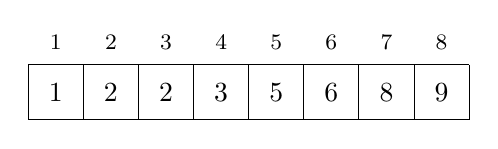
\begin{tikzpicture}[scale=0.7]
\draw (0,0) grid (8,1);
\node at (0.5,0.5) {$1$};
\node at (1.5,0.5) {$2$};
\node at (2.5,0.5) {$2$};
\node at (3.5,0.5) {$3$};
\node at (4.5,0.5) {$5$};
\node at (5.5,0.5) {$6$};
\node at (6.5,0.5) {$8$};
\node at (7.5,0.5) {$9$};

\footnotesize
\node at (0.5,1.4) {$1$};
\node at (1.5,1.4) {$2$};
\node at (2.5,1.4) {$3$};
\node at (3.5,1.4) {$4$};
\node at (4.5,1.4) {$5$};
\node at (5.5,1.4) {$6$};
\node at (6.5,1.4) {$7$};
\node at (7.5,1.4) {$8$};
\end{tikzpicture}
\end{center}

\subsubsection{Järjestämisen alaraja}

Onko sitten mahdollista järjestää taulukkoa
nopeammin kuin ajassa $O(n \log n)$?
Osoittautuu, että tämä \emph{ei} ole mahdollista,
kun rajoitumme
järjestämis\-algoritmeihin,
jotka perustuvat taulukon alkioiden
vertailemiseen.

Aikavaativuuden alaraja on mahdollista todistaa
tarkastelemalla järjestämistä
prosessina, jossa jokainen kahden alkion vertailu
antaa lisää tietoa taulukon sisällöstä.
Prosessista muodostuu seuraavanlainen puu:

\begin{center}
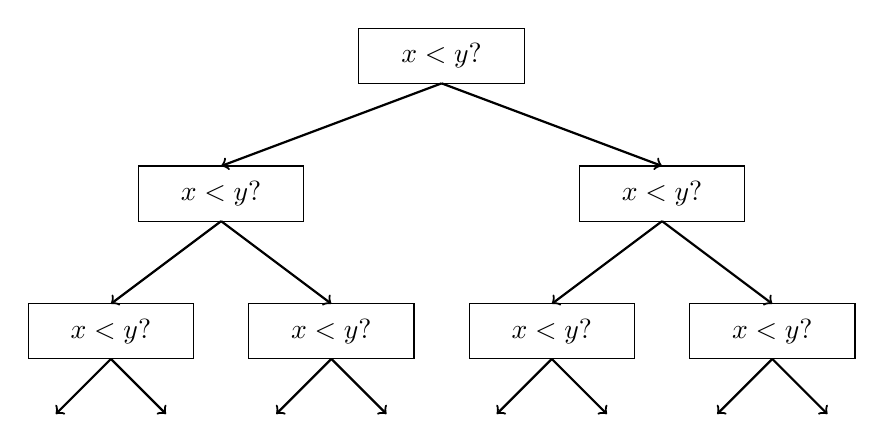
\begin{tikzpicture}[scale=0.7]
\draw (0,0) rectangle (3,1);
\node at (1.5,0.5) {$x < y?$};

\draw[thick,->] (1.5,0) -- (-2.5,-1.5);
\draw[thick,->] (1.5,0) -- (5.5,-1.5);

\draw (-4,-2.5) rectangle (-1,-1.5);
\draw (4,-2.5) rectangle (7,-1.5);
\node at (-2.5,-2) {$x < y?$};
\node at (5.5,-2) {$x < y?$};

\draw[thick,->] (-2.5,-2.5) -- (-4.5,-4);
\draw[thick,->] (-2.5,-2.5) -- (-0.5,-4);
\draw[thick,->] (5.5,-2.5) -- (3.5,-4);
\draw[thick,->] (5.5,-2.5) -- (7.5,-4);

\draw (-6,-5) rectangle (-3,-4);
\draw (-2,-5) rectangle (1,-4);
\draw (2,-5) rectangle (5,-4);
\draw (6,-5) rectangle (9,-4);
\node at (-4.5,-4.5) {$x < y?$};
\node at (-0.5,-4.5) {$x < y?$};
\node at (3.5,-4.5) {$x < y?$};
\node at (7.5,-4.5) {$x < y?$};

\draw[thick,->] (-4.5,-5) -- (-5.5,-6);
\draw[thick,->] (-4.5,-5) -- (-3.5,-6);
\draw[thick,->] (-0.5,-5) -- (0.5,-6);
\draw[thick,->] (-0.5,-5) -- (-1.5,-6);
\draw[thick,->] (3.5,-5) -- (2.5,-6);
\draw[thick,->] (3.5,-5) -- (4.5,-6);
\draw[thick,->] (7.5,-5) -- (6.5,-6);
\draw[thick,->] (7.5,-5) -- (8.5,-6);
\end{tikzpicture}
\end{center}

Merkintä ''$x<y?$'' tarkoittaa taulukon alkioiden
$x$ ja $y$ vertailua.
Jos $x<y$, prosessi jatkaa vasemmalle,
ja muuten oikealle.
Prosessin tulokset ovat taulukon mahdolliset
järjestykset, joita on kaikkiaan $n!$ erilaista.
Puun korkeuden tulee olla tämän vuoksi vähintään
\[ \log_2(n!) = \log_2(1)+\log_2(2)+\cdots+\log_2(n).\]
Voimme arvioida tätä summaa alaspäin
valitsemalla summasta $n/2$
viimeistä termiä ja muuttamalla kunkin
termin arvoksi $\log_2(n/2)$.
Tästä saadaan arvio
\[ \log_2(n!) \ge (n/2) \cdot \log_2(n/2),\]
eli puun korkeus ja sen myötä
pienin mahdollinen järjestämisalgoritmin askelten
määrä on pahimmassa tapauksessa ainakin luokkaa $n \log n$.

\subsubsection{Laskemisjärjestäminen}

\index{laskemisjxrjestxminen@laskemisjärjestäminen}

Järjestämisen alaraja $n \log n$ ei koske algoritmeja,
jotka eivät perustu alkioiden vertailemiseen
vaan hyödyntävät jotain muuta tietoa alkioista.
Esimerkki tällaisesta algoritmista on
\key{laskemisjärjestäminen}, jonka avulla
on mahdollista järjestää
taulukko ajassa $O(n)$ olettaen,
että jokainen taulukon alkio on
kokonaisluku välillä $0 \ldots c$,
missä $c$ on pieni vakio.

Algoritmin ideana on luoda \emph{kirjanpito}, josta selviää,
montako kertaa mikäkin alkio esiintyy taulukossa.
Kirjanpito on taulukko, jonka indeksit ovat alkuperäisen
taulukon alkioita.
Jokaisen indeksin kohdalla lukee, montako kertaa
kyseinen alkio esiintyy alkuperäisessä taulukossa.

Esimerkiksi taulukosta
\begin{center}
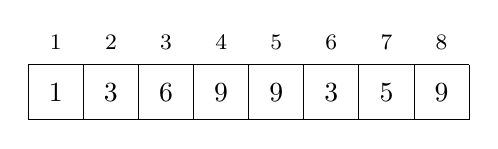
\begin{tikzpicture}[scale=0.7]
\draw (0,0) grid (8,1);
\node at (0.5,0.5) {$1$};
\node at (1.5,0.5) {$3$};
\node at (2.5,0.5) {$6$};
\node at (3.5,0.5) {$9$};
\node at (4.5,0.5) {$9$};
\node at (5.5,0.5) {$3$};
\node at (6.5,0.5) {$5$};
\node at (7.5,0.5) {$9$};

\footnotesize
\node at (0.5,1.4) {$1$};
\node at (1.5,1.4) {$2$};
\node at (2.5,1.4) {$3$};
\node at (3.5,1.4) {$4$};
\node at (4.5,1.4) {$5$};
\node at (5.5,1.4) {$6$};
\node at (6.5,1.4) {$7$};
\node at (7.5,1.4) {$8$};
\end{tikzpicture}
\end{center}
syntyy seuraava kirjanpito:
\begin{center}
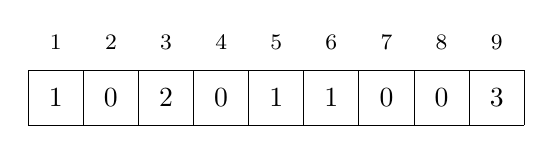
\begin{tikzpicture}[scale=0.7]
\draw (0,0) grid (9,1);
\node at (0.5,0.5) {$1$};
\node at (1.5,0.5) {$0$};
\node at (2.5,0.5) {$2$};
\node at (3.5,0.5) {$0$};
\node at (4.5,0.5) {$1$};
\node at (5.5,0.5) {$1$};
\node at (6.5,0.5) {$0$};
\node at (7.5,0.5) {$0$};
\node at (8.5,0.5) {$3$};

\footnotesize

\node at (0.5,1.5) {$1$};
\node at (1.5,1.5) {$2$};
\node at (2.5,1.5) {$3$};
\node at (3.5,1.5) {$4$};
\node at (4.5,1.5) {$5$};
\node at (5.5,1.5) {$6$};
\node at (6.5,1.5) {$7$};
\node at (7.5,1.5) {$8$};
\node at (8.5,1.5) {$9$};
\end{tikzpicture}
\end{center}

Esimerkiksi kirjanpidossa lukee indeksin 3 kohdalla 2,
koska luku 3 esiintyy kahdesti alkuperäisessä
taulukossa (indekseissä 2 ja 6).

Kirjanpidon muodostus vie aikaa $O(n)$,
koska riittää käydä taulukko läpi kerran.
Tämän jälkeen järjestetyn taulukon luominen
vie myös aikaa $O(n)$, koska kunkin alkion
määrän saa selville suoraan kirjanpidosta.
Niinpä laskemisjärjestämisen
kokonaisaikavaativuus on $O(n)$.

Laskemisjärjestäminen on hyvin tehokas algoritmi,
mutta sen käyttäminen vaatii,
että vakio $c$ on niin pieni,
että taulukon alkioita voi käyttää
kirjanpidon taulukon indeksöinnissä.

\section{Järjestäminen C++:ssa}

\index{sort@\texttt{sort}}

Järjestämisalgoritmia
ei yleensä koskaan kannata koodata itse,
vaan on parempi ratkaisu käyttää
ohjelmointikielen valmista toteutusta.
Esimerkiksi
C++:n standardikirjastossa on funktio \texttt{sort},
jonka avulla voi järjestää helposti taulukoita
ja muita tietorakenteita.

Valmiin toteutuksen käyttämisessä on monia etuja.
Ensinnäkin se säästää aikaa, koska järjestämisalgoritmia
ei tarvitse kirjoittaa itse.
Lisäksi valmis toteutus on varmasti tehokas ja toimiva:
vaikka järjestämisalgoritmin toteuttaisi itse,
siitä tulisi tuskin valmista toteutusta parempi.

Tutustumme seuraavaksi C++:n \texttt{sort}-funktion
käyttämiseen.
Seuraava koodi järjestää vektorin \texttt{v}
luvut pienimmästä suurimpaan:
\begin{lstlisting}
vector<int> v = {4,2,5,3,5,8,3};
sort(v.begin(),v.end());
\end{lstlisting}
Järjestämisen seurauksena
vektorin sisällöksi tulee
$\{2,3,3,4,5,5,8\}$.
Oletuksena \texttt{sort}-funktio järjestää
siis alkiot pienimmästä suurimpaan,
mutta järjestyksen saa käänteiseksi näin:
\begin{lstlisting}
sort(v.rbegin(),v.rend());
\end{lstlisting}
Tavallisen taulukon voi järjestää seuraavasti:
\begin{lstlisting}
int n = 7; // taulukon koko
int t[] = {4,2,5,3,5,8,3};
sort(t,t+n);
\end{lstlisting}
Seuraava koodi taas järjestää merkkijonon \texttt{s}:
\begin{lstlisting}
string s = "apina";
sort(s.begin(), s.end());
\end{lstlisting}
Merkkijonon järjestäminen tarkoittaa,
että sen merkit järjestetään aakkosjärjestykseen.
Esimerkiksi merkkijono ''apina''
on järjestettynä ''aainp''.

\subsubsection{Vertailuoperaattori}

\index{vertailuoperaattori@vertailuoperaattori}

Funktion \texttt{sort} käyttäminen vaatii,
että järjestettävien alkioiden
tietotyypille on määritelty \key{vertailuoperaattori} \texttt{<},
jonka avulla voi selvittää, mikä on kahden alkion järjestys.
Järjestämisen aikana \texttt{sort}-funktio
käyttää operaattoria \texttt{<} aina, kun sen täytyy
vertailla järjestettäviä alkioita.

Vertailuoperaattori on määritelty valmiiksi
useimmille C++:n tietotyypeille,
minkä ansiosta niitä pystyy järjestämään automaattisesti.
Jos järjestettävänä on lukuja, ne järjestyvät
suuruusjärjestykseen,
ja jos järjestettävänä on merkkijonoja,
ne järjestyvät aakkosjärjestykseen.

\index{pair@\texttt{pair}}

Parit (\texttt{pair}) järjestyvät ensisijaisesti
ensimmäisen kentän (\texttt{first}) mukaan.
Jos kuitenkin parien ensimmäiset kentät ovat samat,
järjestys määräytyy toisen kentän (\texttt{second}) mukaan:
\begin{lstlisting}
vector<pair<int,int>> v;
v.push_back({1,5});
v.push_back({2,3});
v.push_back({1,2});
sort(v.begin(), v.end()); // [(1,2),(1,5),(2,3)]
\end{lstlisting}


\index{tuple@\texttt{tuple}}
Vastaavasti \texttt{tuple}-rakenteet
järjestyvät ensisijaisesti ensimmäisen kentän,
toissijaisesti toisen kentän, jne., mukaan:
\begin{lstlisting}
vector<tuple<int,int,int>> v;
v.push_back(make_tuple(2,1,4));
v.push_back(make_tuple(1,5,3));
v.push_back(make_tuple(2,1,3));
sort(v.begin(), v.end()); // [(1,5,3),(2,1,3),(2,1,4)]
\end{lstlisting}

\subsubsection{Omat tietueet}

Jos järjestettävänä on omia tietueita,
niiden vertailuoperaattori täytyy toteuttaa itse.
Operaattori määritellään tietueen sisään
\texttt{operator<}-nimisenä funktiona,
jonka parametrina on toinen alkio.
Operaattorin tulee palauttaa \texttt{true},
jos oma alkio on pienempi kuin parametrialkio,
ja muuten \texttt{false}.

Esimerkiksi seuraava tietue \texttt{P}
sisältää pisteen x- ja y-koordinaatit.
Vertailuoperaattori on toteutettu niin,
että pisteet järjestyvät ensisijaisesti x-koor\-di\-naa\-tin
ja toissijaisesti y-koordinaatin mukaan.

\begin{lstlisting}
struct P {
    int x, y;
    bool operator<(const P &p) {
        if (x != p.x) return x < p.x;
        else return y < p.y;
    }
};
\end{lstlisting}

\subsubsection{Vertailufunktio}

\index{vertailufunktio@vertailufunktio}

On myös mahdollista antaa
\texttt{sort}-funktiolle ulkopuolinen \key{vertailufunktio}.
Esimerkiksi seuraava vertailufunktio
järjestää merkkijonot ensisijaisesti pituuden mukaan
ja toissijaisesti aakkosjärjestyksen mukaan:

\begin{lstlisting}
bool cmp(string a, string b) {
    if (a.size() != b.size()) return a.size() < b.size();
    return a < b;
}
\end{lstlisting}
Tämän jälkeen merkkijonovektorin voi järjestää näin:
\begin{lstlisting}
sort(v.begin(), v.end(), cmp);
\end{lstlisting}

\section{Binäärihaku}

\index{binxxrihaku@binäärihaku}

Tavallinen tapa etsiä alkiota taulukosta
on käyttää \texttt{for}-silmukkaa, joka käy läpi
taulukon sisällön alusta loppuun.
Esimerkiksi seuraava koodi etsii alkiota
$x$ taulukosta \texttt{t}.

\begin{lstlisting}
for (int i = 1; i <= n; i++) {
    if (t[i] == x) // alkio x löytyi kohdasta i
}
\end{lstlisting}

Tämän menetelmän aikavaativuus on $O(n)$,
koska pahimmassa tapauksessa koko taulukko täytyy
käydä läpi.
Jos taulukon sisältö voi olla mikä tahansa,
tämä on kuitenkin tehokkain mahdollinen menetelmä,
koska saatavilla ei ole lisätietoa siitä,
mistä päin taulukkoa alkiota $x$ kannattaa etsiä.

Tilanne on toinen silloin, kun taulukko on
järjestyksessä.
Tässä tapauksessa haku on mahdollista toteuttaa
paljon nopeammin, koska taulukon järjestys
ohjaa etsimään alkiota oikeasta suunnasta.
Seuraavaksi käsiteltävä \key{binäärihaku}
löytää alkion järjestetystä taulukosta
tehokkaasti ajassa $O(\log n)$.

\subsubsection{Toteutus 1}

Perinteinen tapa toteuttaa binäärihaku muistuttaa sanan etsimistä
sanakirjasta. Haku puolittaa joka askeleella hakualueen taulukossa,
kunnes lopulta etsittävä alkio löytyy tai osoittautuu,
että sitä ei ole taulukossa.

Haku tarkistaa ensin taulukon keskimmäisen alkion.
Jos keskimmäinen alkio on etsittävä alkio, haku päättyy.
Muuten haku jatkuu taulukon vasempaan tai oikeaan osaan sen mukaan,
onko keskimmäinen alkio suurempi vain pienempi kuin etsittävä alkio.

Yllä olevan idean voi toteuttaa seuraavasti:
\begin{lstlisting}
int a = 1, b = n;
while (a <= b) {
    int k = (a+b)/2;
    if (t[k] == x) // alkio x löytyi kohdasta k
    if (t[k] > x) b = k-1;
    else a = k+1;
}
\end{lstlisting}

Algoritmi pitää yllä väliä $a \ldots b$, joka on
jäljellä oleva hakualue taulukossa.
Aluksi väli on $1 \ldots n$ eli koko taulukko.
Välin koko puolittuu algoritmin joka vaiheessa,
joten aikavaativuus on $O(\log n)$.

\subsubsection{Toteutus 2}

Vaihtoehtoinen tapa toteuttaa binäärihaku
perustuu taulukon tehostettuun läpikäyntiin.
Ideana on käydä taulukkoa läpi hyppien
ja hidastaa vauhtia, kun etsittävä alkio lähestyy.

Haku käy taulukkoa läpi vasemmalta oikealle aloittaen
hypyn pituudesta $n/2$.
Joka vaiheessa hypyn pituus puolittuu:
ensin $n/4$, sitten $n/8$, sitten $n/16$ jne.,
kunnes lopulta hypyn pituus on 1.
Hyppyjen jälkeen joko haettava alkio on löytynyt
tai selviää, että sitä ei ole taulukossa.

Seuraava koodi toteuttaa äskeisen idean:
\begin{lstlisting}
int k = 1;
for (int b = n/2; b >= 1; b /= 2) {
    while (k+b <= n && t[k+b] <= x) k += b;
}
if (t[k] == x) // alkio x löytyi kohdasta k
\end{lstlisting}

Muuttuja $k$ on läpikäynnin kohta taulukossa
ja muuttuja $b$ on hypyn pituus.
Jos alkio $x$ esiintyy taulukossa,
sen kohta on muuttujassa $k$ algoritmin päätteeksi.
Algoritmin aikavaativuus on $O(\log n)$,
koska \texttt{while}-silmukassa oleva koodi suoritetaan
aina enintään kahdesti.

\subsubsection{Muutoskohdan etsiminen}

Käytännössä binäärihakua tarvitsee toteuttaa
harvoin alkion etsimiseen taulukosta,
koska sen sijasta voi käyttää standardikirjastoa.
Esimerkiksi C++:n funktiot \texttt{lower\_bound}
ja \texttt{upper\_bound} toteuttavat binäärihaun
ja tietorakenne \texttt{set} ylläpitää joukkoa,
jonka operaatiot ovat $O(\log n)$-aikaisia.

Sitäkin tärkeämpi binäärihaun käyttökohde on 
funktion \key{muutoskohdan} etsiminen.
Oletetaan, että haluamme löytää pienimmän arvon $k$,
joka on kelvollinen ratkaisu ongelmaan.
Käytössämme on funktio $\texttt{ok}(x)$,
joka palauttaa \texttt{true}, jos $x$ on kelvollinen
ratkaisu, ja muuten \texttt{false}.
Lisäksi tiedämme, että $\texttt{ok}(x)$ on \texttt{false}
aina kun $x<k$ ja \texttt{true} aina kun $x \geq k$.
% Toisin sanoen haluamme löytää funktion \texttt{ok} \emph{muutoskohdan},
% jossa arvosta \texttt{false} tulee arvo \texttt{true}.
Tilanne näyttää seuraavalta:

\begin{center}
\begin{tabular}{r|rrrrrrrr}
$x$ & 0 & 1 & $\cdots$ & $k-1$ & $k$ & $k+1$ & $\cdots$ \\
\hline
$\texttt{ok}(x)$ & \texttt{false} & \texttt{false}
& $\cdots$ & \texttt{false} & \texttt{true} & \texttt{true} & $\cdots$ \\
\end{tabular}
\end{center}

\noindent
Nyt muutoskohta on mahdollista etsiä käyttämällä
binäärihakua:

\begin{lstlisting}
int x = -1;
for (int b = z; b >= 1; b /= 2) {
    while (!ok(x+b)) x += b;
}
int k = x+1;
\end{lstlisting}

Haku etsii suurimman $x$:n arvon,
jolla $\texttt{ok}(x)$ on \texttt{false}.
Niinpä tästä seuraava arvo $k=x+1$
on pienin arvo, jolla $\texttt{ok}(k)$ on \texttt{true}.
Hypyn aloituspituus $z$ tulee olla 
sopiva suuri luku, esimerkiksi sellainen,
jolla $\texttt{ok}(z)$ on varmasti \texttt{true}.

Algoritmi kutsuu $O(\log z)$ kertaa funktiota
\texttt{ok}, joten kokonaisaikavaativuus
riippuu siitä, kauanko funktion \texttt{ok}
suoritus kestää.
Esimerkiksi jos ratkaisun tarkastus
vie aikaa $O(n)$, niin kokonaisaikavaativuus
on $O(n \log z)$.

\subsubsection{Huippuarvon etsiminen}

Binäärihaulla voi myös etsiä
suurimman arvon funktiolle,
joka on ensin kasvava ja sitten laskeva.
Toisin sanoen tehtävänä on etsiä arvo
$k$ niin, että

\begin{itemize}
\item
$f(x)<f(x+1)$, kun $x<k$, ja
\item
$f(x)>f(x+1)$, kun $x >= k$.
\end{itemize}

Ideana on etsiä binäärihaulla
viimeinen kohta $x$,
jossa pätee $f(x)<f(x+1)$.
Tällöin $k=x+1$,
koska pätee $f(x+1)>f(x+2)$.
Seuraava koodi toteuttaa haun: 

\begin{lstlisting}
int x = -1;
for (int b = z; b >= 1; b /= 2) {
    while (f(x+b) < f(x+b+1)) x += b;
}
int k = x+1;
\end{lstlisting}

Huomaa, että toisin kuin tavallisessa binäärihaussa,
tässä ei ole sallittua,
että peräkkäiset arvot olisivat yhtä suuria.
Silloin ei olisi mahdollista tietää,
mihin suuntaan hakua tulee jatkaa.



